\documentclass[twocolumn]{article}
% Turkish manuscript source - compiled with pdflatex + bibtex (apalike)

% Turkish language and font support
\usepackage[T1]{fontenc}
\usepackage[utf8]{inputenc}
\usepackage{lmodern}
\usepackage[shorthands=off,turkish]{babel}

% Essential packages
\usepackage{hyperref}
\usepackage{graphicx}
\graphicspath{{figures/}{../figures/}}
\usepackage{amsmath}
\usepackage{amssymb}
\usepackage{booktabs}
\usepackage[style=english,autostyle=false]{csquotes}
\usepackage[backend=bibtex,style=authoryear,natbib=true,maxcitenames=2]{biblatex}
\addbibresource{references.bib}
\usepackage{appendix}

% Page geometry
\usepackage[letterpaper,
            includeheadfoot,
            layoutsize={8.125in,10.875in},
            layouthoffset=0.1875in,
            layoutvoffset=0.0625in,
            left=38.5pt,
            right=43pt,
            top=43pt,
            bottom=44pt,
            headheight=0pt,
            headsep=-2pt,
            columnsep=0.3125in,
            footskip=25pt,
            marginparwidth=38pt]{geometry}

% Authors and affiliations
\usepackage{authblk}

% Float control
\renewcommand{\topfraction}{0.9}
\renewcommand{\bottomfraction}{0.9}
\renewcommand{\textfraction}{0.05}
\renewcommand{\floatpagefraction}{0.9}

% Math operators
\DeclareMathOperator*{\mean}{mean}
\DeclareMathOperator*{\std}{std}
\DeclareMathOperator*{\AbsDiff}{AbsDiff}

% Bibliography settings
\setlength{\bibitemsep}{0pt plus 0.3ex}

% First page footer
\usepackage{fancyhdr}
\fancypagestyle{firstpage}{%
  \fancyhf{}%
  \fancyfoot[C]{\footnotesize
    Bu sürüm hakem değerlendirmesinden geçmemiştir. Görüş ve geri bildirimlere açığız.}%
  \renewcommand{\headrulewidth}{0pt}%
}

% Caption formatting
\usepackage{caption}
\captionsetup{labelfont=bf, font=small}

% Author/affiliation fonts
\renewcommand\Authfont{\large}
\renewcommand\Affilfont{\normalsize}
\renewcommand\Authand{ ve }
\renewcommand\Authands{ ve }

% Autoref customization
\renewcommand{\tableautorefname}{Tab.}
\renewcommand{\figureautorefname}{Şek.}
\renewcommand{\equationautorefname}{Denk.}
\renewcommand{\appendixautorefname}{Ek}

\title{\LARGE LLM İşe Alım Kararlarında Warmth ve Competence Temsillerinin Probing Yöntemiyle İncelenmesi}
\date{\today}
\author[1]{Emrecan Ulu}
\author[2]{Jorge Lastra Cerda}
\affil[1]{University of Konstanz}
\affil[2]{University of Konstanz}

\begin{document}
\twocolumn[
  \begin{@twocolumnfalse}
\maketitle
\thispagestyle{firstpage}

\begin{abstract}
\noindent
İşe alım süreçlerindeki ayrımcılık hem insanlar hem de büyük dil modelleri
üzerinde belgelenmiş olsa da bu ayrımcılığı üreten iç mekanizmalar yeterince
anlaşılmış değildir. Bu çalışmada Stereotype Content Model'in warmth ve
competence boyutlarının, açık ağırlıklı ve instruction-tuned dört dil modelinin
(Gemma-3-12B, Gemma-3-27B, Llama-3.1-8B ve Qwen3-14B) residual stream'lerinde
doğrusal yönler olarak kodlanıp kodlanmadığını ve bu temsiller doğrudan
steering ile değiştirildiğinde işe alım callback önerilerini nedensel olarak
değiştirip değiştirmediğini probing yöntemiyle inceliyoruz. Warmth ve
competence'ın dört mimarinin tamamında çok büyük effect size değerleriyle
doğrusal olarak ayrılabildiğini, yönlerin concept-level yargılarda nedensel
işlev taşıdığını ve Gemma ailesinin insan sosyal algı puanlarıyla kısmen
hizalanırken Llama ile Qwen'in warmth anti-alignment gösterdiğini buluyoruz.
Temsilden işe alım kararına uzanan nedensel zincir kırılgan ve modele bağlıdır:
concept-level düzeyde steering'e en açık model anlamlı bir mediation path
göstermezken, daha büyük Gemma modeli insanlardaki ırksal callback farkını bir
standard deviation'dan fazla tersine çevirmektedir. Bu sonuç, devralınmış
ayrımcılıktan çok instruction-tuning kaynaklı bir overcorrection ile tutarlıdır.
\vspace{0.50cm}
\end{abstract}
  \end{@twocolumnfalse}
]

\renewcommand{\thefootnote}{\fnsymbol{footnote}}
\footnotetext[0]{Sorumlu yazarlar: emrecan.ulu@uni-konstanz.de; jorge.lastra-cerda@uni-konstanz.de}
\renewcommand{\thefootnote}{\arabic{footnote}}
\setcounter{footnote}{0}

% -----------------------------------------------------------------------------
\section*{Giriş}
% -----------------------------------------------------------------------------

AI destekli araçlar günümüzde özgeçmişleri taramakta, adayları sıralamakta ve
modern işe alım sürecinin her aşamasında callback kararlarını desteklemektedir.
SHRM'nin 2025 Talent Trends araştırmasına göre ABD'deki kuruluşların yarısı işe
alımı desteklemek için AI kullanmakta, yüzde 44'ü ise bu teknolojiyi özellikle
özgeçmiş taraması için devreye almaktadır \citep{shrm2025talent}. Bu ölçekte,
model önerilerindeki her sistematik sapma işe erişimde doğrudan eşitsizliğe
dönüşür.

Bu sapma varsayımsal değildir. On yıllara yayılan correspondence study'ler;
ırk, ulusal köken, yaş, engellilik ve gender eksenlerinde ölçülebilir işe alım
ayrımcılığı bulunduğunu göstermiştir \citep{bertrand2004emily,
oreopoulos2011why, neumark2019older, correll2007getting, tilcsik2011pride,
ameri2018disability}. İşe alım kararını otomatikleştirmenin bu örüntüleri
koruyup korumadığı ya da büyütüp büyütmediği artık güncel bir araştırma
sorusudur. Büyük dil modellerine ilişkin çeşitli behavioral audit çalışmaları
bunun gerçekleştiğine işaret etmektedir: \citet{wilson2024gender} ve
\citet{chaturvedi2025callback}, LLM'lerin özgeçmiş değerlendirmesinde bazı
demografik grupları sistematik olarak diğerlerinden üstün tuttuğunu bulurken;
\citet{an2024llm}, \citet{an_measuring_2025} ve \citet{gaebler2024auditing},
GPT ailesinin callback önerilerinde kalıcı ırk ve gender farkları
belgelemektedir. Bu çalışmalar bias'ın varlığı konusunda birleşmekte, fakat
yönü ve büyüklüğü konusunda ayrışmaktadır. Hiçbiri iç mekanizmanın yerini
belirleyemez; modelin neye karar verdiğini betimler, bu karara nasıl ulaştığını
değil.

Mechanistic interpretability bu mekanizmayı incelemek için bir yol sunar. Word
embedding araştırmaları, semantik concept'lerin yüksek boyutlu activation
space içinde doğrusal yönler hâlinde kümelendiğini göstermiş
\citep{mikolov2013word2vec}; linear representation hypothesis ise bu görüşü
modern büyük modeller için biçimselleştirmiştir \citep{park2024linear}.
Representation engineering \citep{zou2023repeng} ve activation addition
\citep{turner2023activation}, bir modeli böyle bir yön boyunca steering ile
değiştirmenin davranışı nedensel olarak değiştirdiğini göstermiş; circuit
analizleri de tekil bileşenleri tanınabilir hesaplamalarla ilişkilendirmiştir
\citep{olah2020zoom}. Yakın zamanda \citet{sofroniew2026emotion}, Claude
Sonnet'teki emotion concept'lerinin doğrusal residual-stream yönleri olarak
kodlandığını ve doğrudan steering altında davranışı nedensel olarak
düzenlediğini göstermiştir. Bu bulgu, representation geometry'nin sembolik
word vector'lerden instruction-tuned modellerin iç activation'larına kadar
uzandığına dair kanıt sunar. Biz bu tekniği farklı bir construct'a uyguluyoruz.

Bu construct, Stereotype Content Model'e göre sosyal grupların algılandığı iki
eksen olan warmth ve competence'tır \citep{fiske2002model}. Sosyal işaretlere
ilişkin warmth ve competence puanları, Kuzey Amerika'da onlarca yıla yayılan
correspondence study'lerdeki insan callback oranlarını yordamaktadır
\citep{gallo2024warmth}; dolayısıyla bu eksenler LLM işe alım eşitsizlikleri
için doğal bir aday mekanizmadır. Açık ağırlıklı dört modelin warmth ve
competence'ı doğrusal olarak decode edilebilen residual-stream yönleri hâlinde
içselleştirip içselleştirmediğini, bu yönlerin nedensel işlev taşıyıp
taşımadığını ve eşleştirilmiş bir insan benchmark'ına karşı gözlemlediğimiz
isim kaynaklı callback farklarına aracılık edip etmediğini soruyoruz. Bu soru,
yanlış kararların sonuçlarının doğrudan ve ölçülebilir olduğu bir alanda
mechanistic interpretability'yi correspondence study geleneğiyle birleştirir.

% -----------------------------------------------------------------------------
\section*{Arka Plan: Bir Dil Modelindeki Concept Nasıl Okunur?}
% -----------------------------------------------------------------------------

\paragraph{Activation'lar ve Residual Stream.}
Bir transformer'daki her forward pass, hesaplamayı toplamsal residual
connection'lar üzerinden biriktirir: her layer~$\ell$,
$d_{\mathrm{model}}$ boyutlu bir $h_\ell \in
\mathbb{R}^{d_{\mathrm{model}}}$ state'ini okur ve
$h_{\ell+1} = h_\ell + f_\ell(h_\ell)$ biçiminde güncellenmiş bir sürümünü
yazar. Burada $f_\ell$, ilgili layer'ın attention ve MLP sub-block
çıktılarının birleşimidir. Circuit-level analizler, düşük düzeyli syntax'tan
yüksek düzeyli semantic content'e kadar belirli feature'ların bu stream içinde
context'ler arasında tutarlı geometric pattern'ler olarak yerelleştiğini
göstermiştir \citep{olah2020zoom}. Mimarinin tamamını probing ile incelemek
yerine, seçilmiş tek bir depth'teki residual-stream state'ini çıkarıyor ve bu
vector'ü warmth ile competence'ın yönler olarak bulunduğu space kabul ediyoruz.
Bu depth, Cohen's~$d$ emergence curve'lerine göre seçilen network layer'larının
yaklaşık yüzde 65'ine karşılık gelir.

\paragraph{Yönler Olarak Concept'ler.}
Semantic content'in doğrusal yönler hâlinde düzenlendiği sezgisi word-embedding
analojilerine dayanır \citep{mikolov2013word2vec}. \textit{Linear
representation hypothesis} \citep{park2024linear}, bu sezgiyi büyük
transformer modelleri için biçimselleştirir: high-level feature'lar
residual-stream space içindeki yönlere karşılık gelir ve bir representation'ın
bu yöne projection'ı, ilgili feature'ın ne kadar güçlü bulunduğunu ölçen bir
scalar üretir. Hedef concept için böyle bir yön çıkarmak amacıyla, concept'i
ifade eden metinlerden (condition~$A$) ve etmeyen eşleştirilmiş metinlerden
(condition~$B$) residual-stream activation'ları topluyor ve mean-difference'ı
hesaplıyoruz:
\begin{equation}
  v = \bar{h}_{A} - \bar{h}_{B}.
  \label{eq:mean_diff}
\end{equation}
$\hat{v}$ yönüne normalization uygulandığında bir concept direction elde edilir;
yeni bir metnin concept score'u $\hat{v}^{\!\top} h$ olur. Cross-validated
classification ve topic-holdout accuracy ile burada doğruladığımız temel iddia,
bu yönün oluşturulmasında kullanılan belirli metinlerin ötesine genellenmesidir
(\autoref{fig:concept_geometry}).

\begin{figure}[t]
\centering
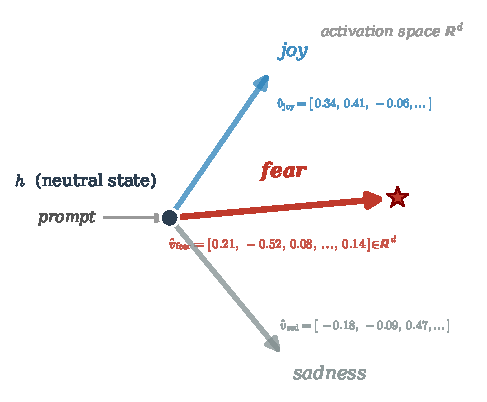
\includegraphics[width=0.85\columnwidth]{background_emotion_vector.pdf}
\caption{\textbf{Activation space içinde yönler olarak emotion vector'ler (şematik).}
Her emotion, nötr bir model state'i olan~$h$ noktasından çıkan bir unit direction'a
karşılık gelir. Fear uyandıran bir prompt verildiğinde residual stream,
$\hat{v}_{\text{fear}}$ boyunca kayar; bu yön burada temsili $d$ boyutlu
coordinate'leriyle kodlanmıştır. \citet{sofroniew2026emotion} temel alınmıştır;
construct'ı değil, geometry'yi yeniden kullanıyoruz.}
\label{fig:emotion_vector}
\end{figure}

\begin{figure}[t]
\centering
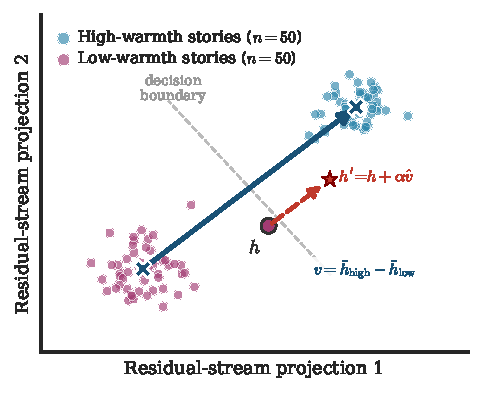
\includegraphics[width=0.85\columnwidth]{background_concept_geometry.pdf}
\caption{\textbf{Residual-stream concept geometry (şematik).}
Mean-difference yönü $v = \bar{h}_{\mathrm{high}} -
\bar{h}_{\mathrm{low}}$ ile ayrılan iki story cluster (mavi ok).
Kırmızı kesikli ok, marjinal bir noktayı decision boundary'nin ötesine taşıyan
tek bir steering adımını, $h' = h + \alpha\,\hat{v}$, gösterir.
Gösterim ölçülmüş verilere değil, sentetik activation'lara dayanır.}
\label{fig:concept_geometry}
\end{figure}

\paragraph{Correlation'dan Causation'a.}
Mean-difference yöntemiyle çıkarılan bir yön başlangıçta correlational'dır:
high ve low condition activation'larını ayırır, ancak modelin bu yönü nedensel
olarak kullandığını tek başına göstermez. Causality'yi test etmek için inference
sırasında residual stream'e müdahale ediyoruz. Probe layer'da modelin iç
state'ini şu ifadeyle değiştiriyoruz:
\begin{equation}
  h' = h + \alpha\,\hat{v},
  \label{eq:steering}
\end{equation}
Burada $\alpha$, müdahalenin büyüklüğünü ve yönünü kontrol eden signed
scalar'dır. Orthogonal bir control direction benzer bir değişim üretmezken
modelin downstream davranışı $\alpha$ ile sistematik biçimde değişiyorsa, söz
konusu yön modelin hesaplamalarına nedensel olarak katılmaktadır. Activation
addition \citep{turner2023activation} ve representation engineering
\citep{zou2023repeng}, bu yaklaşımı temellendirmiş ve çeşitli model ve hedef
davranışlarda ampirik destek sağlamıştır.

\paragraph{Emotion-Vector Template'i.}
\citet{sofroniew2026emotion}, bu framework'ü Claude Sonnet'teki emotion
concept'lerine uygulamıştır. Her emotion için contrastive text pair'leri
oluşturmuş, residual stream'de mean-difference yönleri çıkarmış, modeli bu
yönler boyunca steering ile değiştirmiş ve davranışta sistematik, yorumlanabilir
değişimler gözlemlemişlerdir. Çalışma ayrıca, direction vector'lerden genel
evaluative valence'ı kaldıran neutral-corpus PCA denoising prosedürünü
tanıtmıştır. Methods bölümünde açıkladığımız üzere, warmth ve competence
content'ini ortak narrative polarity'den ayırmak için bu adımı aynen
uyguluyoruz. Geometry ve method'u yeniden kullanıyor, farklı bir construct'ı
inceliyoruz. Warmth ve competence, Stereotype Content Model'den gelen social
perception dimension'larıdır; emotion state'leri değildir. Bu nedenle kendi
direction vector'lerimizi ``emotion vector'' olarak adlandırmak bir category
error olur. \autoref{fig:emotion_vector}, temel fikri gösterir: her emotion,
residual-stream space içinde çıkarılabilen, incelenebilen ve model steering'inde
kullanılabilen sayısal bir representation'a sahip ayrı bir yöndedir.

% -----------------------------------------------------------------------------
\section*{Neden Warmth ve Competence, Neden İşe Alım ve Hangi Veriler?}
% -----------------------------------------------------------------------------

\paragraph{Construct.}
Stereotype Content Model \citep{fiske2002model}, social perception'ın iki temel
eksen boyunca düzenlendiğini öne sürer: algılanan intentions ve
trustworthiness'ü kapsayan warmth ile algılanan ability ve effectiveness'ı
kapsayan competence. Bu iki dimension birlikte, insanların social group ve
individual değerlendirmelerindeki variance'ın önemli bir bölümünü açıklar
\citep{fiske2007universal}.

\paragraph{İşe Alımla Bağlantı.}
\citet{gallo2024warmth}, kritik ampirik köprüyü sağlar. Kuzey Amerika'da
yayımlanmış on correspondence study'de 787 rater tarafından 282 applicant first
name için verilen 24.220 warmth ve competence rating'ini birleştiren yazarlar,
algılanan warmth ve competence'ın bu isimlerin gerçek işe alım deneylerinde
aldığı callback oranlarını güvenilir biçimde yordadığını göstermektedir. Human
benchmark bu nedenle nadir bir olanak sunar: probing ile incelediğimiz social
perception dimension'ları ile gerçek labor market outcome'ları arasında doğrudan
quantitative bir bağlantı. LLM'lere ilişkin behavioral audit'ler isim kaynaklı
işe alım farklarını belgelemiştir \citep{an2024llm, an_measuring_2025,
gaebler2024auditing}; fakat hiçbiri model içindeki warmth ve competence
representation'larının bu signal'ı taşıyıp taşımadığını test etmemiştir. Gallo
ve Hausladen dataset'ini hem probe'larımız için external validity check hem de
model-level disparity'leri karşılaştırmak için reference olarak kullanıyoruz.

\paragraph{Bu Verilerin Seçilme Nedeni.}
Warmth ve competence'ı doğrudan hiring prompt'larından probing ile çıkarmak,
social perception dimension'larını işe alım kararının kendisiyle confound ederdi.
Representation'ları izole etmek için, warmth ve competence'ı ifade eden ancak
hedef construct'la karıştırılabilecek demographic identity cue'ları içermeyen
metinlere ihtiyaç vardır. Pilot çalışma, bu constraint olmadan LLM ile üretilen
concept story'lerin low-warmth ve low-competence condition'larına sistematik
olarak erkek ve Anglo isimli protagonist'ler atadığını göstermiştir. Böyle bir
örüntü, herhangi bir işe alım değerlendirmesi başlamadan demographic
expectation'ları direction vector'lere yerleştirirdi. Bu nedenle 200 concept
story'nin tamamında isimsiz ve gender-neutral bir protagonist bulunur; vector'ler
yalnızca betimlenen behavior'dan oluşturulur. Hiring evaluation ise ayrı bir
stimulus set kullanır: \citet{gallo2024warmth} çalışmasındaki 282 applicant name,
name'in değişen tek signal olması için aynı sabit application ile eşleştirilir.
Bu 282 name'in 149'u aynı kaynaktaki yayımlanmış per-name callback dataset'inde
de bulunur ve ABD race ile gender label'larına sahiptir; demographic disparity
için benchmark comparison bu 149 name üzerinde yapılır. Her name'in crowdsourced
perception rating'i bulunduğu için, yayımlanmış callback verisi olmayanlar da
dahil olmak üzere 282 name'in tamamı probe-versus-human warmth ve competence
rating alignment analizinde kullanılır.

% -----------------------------------------------------------------------------
\section*{Yöntem}
% -----------------------------------------------------------------------------

\paragraph{Story Corpus.}
Demographic identity'den bağımsız concept direction vector'leri oluşturmak için,
dört condition'a eşit dağıtılmış 200 kısa narrative ürettik: high warmth, low
warmth, high competence ve low competence (condition başına 50 story). Her biri
yaklaşık 90--150 word uzunluğundaydı. Story'ler, on domain'e yayılan 50 farklı
gündelik topic çevresinde yazıldı (workplace, learning, community, sport, travel
ve diğerleri). Situational vocabulary'nin high ve low pole'lar arasında dengeli
olması için her topic her condition'da bir kez yer aldı. Bütün story'lerde
isimsiz, gender-neutral ve third-person bir protagonist (``they'') bulunur. Bu
tasarım kararı, AI ile üretilen concept story'lerde sistematik demographic skew
gösteren pilot çalışmaya dayanır: low-warmth ve low-competence condition'ları
büyük ölçüde erkek, Anglo isimli protagonist'lere; high condition'lar ise kadın
ve demografik açıdan çeşitli protagonist'lere atanmıştı. Neutralisation olmadan
direction vector'ler hedef social dimension ile birlikte demographic
expectation'ları da kodlar ve incelemeyi amaçladığımız bias ile probe'u confound
ederdi. Identity signal'larının tümüyle kaldırılması sayesinde her story'nin
activation'ı group membership yerine betimlenen behavior tarafından belirlenir.
Story'ler bir large language model tarafından üretildi ve forbidden-vocabulary
violation, condition'lar arası length balance ve demographic neutrality için
automated check'lerle doğrulandı. AI-generated stimulus kullanımı circularity
endişesi doğurmaktadır; bu konuyu Limitations bölümünde ele alıyoruz. Mevcut 200
story'lik corpus bir pilot'tur; data collection ilerledikçe 400 story'ye
genişletmeyi planlıyoruz.

\paragraph{Activation Extraction.}
Dört açık ağırlıklı instruction-tuned modelden residual-stream activation'ları
çıkarmak için TransformerLens \citep{nanda2022transformerlens} kullandık:
primary model Gemma-3-12B-it \citep{gemmateam2025gemma3}, within-family scale
replication için Gemma-3-27B-it ve cross-architecture replication için Qwen3-14B
\citep{qwen2025qwen3} ile Llama-3.1-8B-Instruct
\citep{grattafiori2024llama3}. Her modelde full layer sweep'ten elde edilen
Cohen's~$d$ emergence curve'leri temelinde seçilen ve model depth'inin yaklaşık
yüzde 65'ine karşılık gelen layer'daki post-layer residual-stream state'ini
kaydettik. \autoref{tab:models}, her modelin tam probe layer'ını, model width'ini
ve mean residual-stream norm'unu gösterir. Her story için activation'lar prompt
prefix'i atlanarak position~50 sonrasındaki token position'larında mean pooling
ile birleştirildi ve story başına tek bir $d_\mathrm{model}$ boyutlu vector elde
edildi. Warmth ve competence direction vector'leri daha sonra mean-difference
olarak oluşturuldu:
$v_W = \bar{x}_\mathrm{high\,warmth} - \bar{x}_\mathrm{low\,warmth}$
ve
$v_C = \bar{x}_\mathrm{high\,comp.} - \bar{x}_\mathrm{low\,comp.}$.
Cross-architecture comparison'ı mümkün kılmak için dört model de tamamen aynı
condition'larda çalıştırıldı (aynı story'ler, aynı pooling rule, aynı seed
20260527).

\begin{table}[t]
\centering
\small
\caption{%
  Model parameter'ları ve probe extraction setting'leri.
  Probe layer, seçilen/toplam layer olarak verilmiştir.
  $\bar{\|h\|}$, steering intervention'larının scale'ini belirleyen probe
  layer'daki mean residual-stream norm'dur; model activation scale'leri
  arasındaki orders-of-magnitude fark, normalization olmadan raw-strength
  comparison'larını anlamsız kılar.
}
\label{tab:models}
\begin{tabular}{lcccc}
\toprule
Model & $d_\mathrm{model}$ & Probe layer & $\bar{\|h\|}$ \\
\midrule
Gemma-3-12B-it          & 3840 & 31/48 & 79{,}722 \\
Gemma-3-27B-it          & 5376 & 40/62 & 61{,}576 \\
Llama-3.1-8B-Instruct   & 4096 & 20/32 & 11.4     \\
Qwen3-14B               & 5120 & 26/40 & 206.6    \\
\bottomrule
\end{tabular}
\end{table}

\paragraph{PCA Denoising.}
Warmth ve competence direction vector'leri general narrative valence'ı yansıtan
önemli bir ortak component paylaşır: protagonist'i olumlu betimleyen story'ler,
ister warm ister competent olsun, residual stream'in benzer bir bölgesinde yer
alır; negative valence'a sahip story'ler için de aynı durum geçerlidir.
Conceptual content'i evaluative polarity'den ayırmak için
\citet{sofroniew2026emotion} çalışmasının neutral-corpus denoising prosedürünü
izliyoruz. Concept story'lerle length-matched (90--200 word), emotionally charged
ya da violent content içermeyecek biçimde filtrelenmiş 1.500 Wikipedia giriş
paragrafından oluşan neutral corpus kuruyoruz. Residual-stream activation'lar
aynı layer ve pooling rule ile çıkarılır. Principal component analysis (PCA) bu
neutral activation'lar üzerinde fit edilir; neutral variance'ın en az yüzde
50'sini birlikte açıklayan top component'ler daha sonra iki direction vector'den
de project out edilir. Gemma-3-12B'de ilk principal component tek başına neutral
variance'ın yüzde 56,1'ini açıklar; bu component'in çıkarılması warmth ve
competence vector'leri arasındaki cosine'ı 0,749'dan 0,530'a düşürür.
Gemma-3-27B'de yüzde 50 threshold'unu geçmek için 43 component gerekir (açıklanan
variance yüzde 50,2) ve inter-axis cosine 0,708'den 0,487'ye düşer. Denoising
sonrasında kalan cosine değerleri (sırasıyla 0,53 ve 0,49), insan rating'lerinde
gözlenen gerçek warmth-competence correlation'ı ile tutarlıdır
($r \approx 0.61$; \citealt{fiske2002model}). Bu durum residual overlap'in bir
denoising failure yerine gerçek conceptual co-variation'ı yansıttığını düşündürür.
Elde edilen denoised vector'ler bütün causal steering experiment'larında
kullanılır.

\paragraph{Probe Validation.}
Her direction vector'ün validity'sini birbirini tamamlayan beş metric ile
değerlendiriyoruz. (i)~\textit{5-fold cross-validated accuracy}: bir logistic
regression classifier her target contrast içindeki full residual-stream
representation'lar üzerinde train edilir ve accuracy beş stratified fold
üzerinden average edilir. (ii)~\textit{Topic-holdout accuracy}: GroupKFold
kullanan daha sıkı bir variant'tır. Belirli bir topic'e ait bütün story'ler aynı
fold'a atanır; böylece probe'un yalnızca tanıdık topic'lerin görülmemiş
phrasing'lerine değil, bütünüyle yeni situation'lara genellenip genellenmediği
test edilir. (iii)~\textit{Cohen's $d$}: direction vector'e yapılan projection'ın
high ve low condition'ları arasındaki standardized mean difference, 1.000 random
unit vector'den oluşan empirical null distribution ile karşılaştırılır.
(iv)~\textit{Split-half cosine stability}: her condition'daki 50 story random
olarak 25'er story'lik iki parçaya ayrılır; her parçadan bir direction hesaplanır
ve aralarındaki cosine raporlanır. (v)~\textit{Cross-axis classification}:
fold-local standardized projection'larla warmth direction'ın competence label'ı
ve tersini yordayıp yordamadığını test ederek shared evaluative content düzeyini
ölçeriz. Dört modelin ortak bir cross-architecture construct üzerinde birleşip
birleşmediğini sınamak için model pair'leri arasında per-story Spearman rank
correlation da hesaplanır.

\paragraph{Causal Steering.}
Çıkarılan yönlerin model behavior'ı ile yalnızca correlate olmak yerine onu
nedensel olarak etkileyip etkilemediğini test etmek için, probe layer'da
TransformerLens hook'ları üzerinden activation steering
\citep{turner2023activation} uyguluyoruz. Steering strength, söz konusu
layer'daki mean residual-stream norm'a göre ifade edilir; böylece activation
scale'leri orders of magnitude düzeyinde farklılaşan modeller karşılaştırılabilir
(\autoref{tab:models} içindeki $\bar{\|h\|}$ değerlerine bakınız).
\textit{Concept-level} evaluation'da model, held-out topic'lerde ``Is the
protagonist high in warmth/competence? Answer only Yes or No'' sorusunu yanıtlar
(topic index ile belirlenen 40 training / 10 test). Local regime, mean norm ile
çarpılan $\alpha \in \{-0.10,\,-0.05,\,0,\,+0.05,\,+0.10\}$ değerlerini
kullanır. Outcome, next-token logit margin
$\Delta = \mathrm{logit}(\text{Yes}) - \mathrm{logit}(\text{No})$ olarak
tanımlanır. \textit{Hiring-level} evaluation'da aynı hook'lar, applicant
roster'ından 60 name içeren subset üzerinde resume-evaluation prompt'ları
işlenirken uygulanır. Broad sweep $\alpha \in \{\pm 0.25,\,\pm 0.50\}$,
iki Gemma modeli için local-regime follow-up ise $\{\pm 0.05,\,\pm 0.10\}$
değerlerini kullanır; outcome callback logit margin'dır. Altı direction test
ediyoruz: dense target direction, decoded Gemma Scope~2 SAE direction
\citep{deepmind2025gemmascope2}, axis-specific component, shared component,
opposing concept axis ve random orthogonal control. Uncertainty, paired topic
bootstrap resampling ile tahmin edilir.

\paragraph{Hiring Evaluation.}
Hiring stimulus'ları, \citet{gallo2024warmth} çalışmasındaki 282 applicant first
name'i sabit bir administrative-assistant application ile birleştirir. Education,
experience ve skills bütün trial'larda aynıdır; değişen tek signal name'dir.
Model ``would you recommend calling this candidate back for an interview? Answer
with a single word: Yes or No'' sorusunu yanıtlar. Outcome olan
\textit{callback margin}, next-token logit farkı
$\mathrm{logit}(\text{Yes}) - \mathrm{logit}(\text{No})$ olarak tanımlanır.
Race ve gender label'ları modele hiçbir zaman gösterilmez; human correspondence
study tasarımını yansıtacak biçimde \citet{gallo2024warmth} coding'inden post
hoc atanır \citep{bertrand2004emily}. Hiring prompt'ından bağımsız olarak her
name neutral bir carrier sentence içine yerleştirilir ve residual-stream
activation'ı warmth ile competence direction'larına project edilir. Böylece elde
edilen per-name probe score'lar, 787 rater'ın on source study'deki 24.220
judgement'ından aggregate edilen human rating'lerle Spearman rank correlation
kullanılarak karşılaştırılır.

\paragraph{Disparity ve Mediation.}
Group-level disparity'ler, name group'ları arasındaki mean callback margin
farklarıdır (race: Black-signalling 47 ve White-signalling 180 name; gender:
female 154 ve male 115 name). Farklı logit scale'lere sahip modelleri
karşılaştırabilmek için değerler within-model callback-margin standard deviation
ile standardized edilir. Human reference gap'ler, benchmark ile first name
üzerinden eşleşen 149 name'deki yayımlanmış per-name callback rate'lerden
aggregate edilir. İç warmth ve competence representation'larının name-group
signal'ını callback decision'a taşıyıp taşımadığı, name group $\to$ probe score
$\to$ callback margin path'i üzerindeki bootstrap mediation ile test edilir
(5.000 resample, seed 20260527, complete data içeren $n = 269$ name, race subset
$n = 227$). On altı model-by-grouping-by-probe combination'ın tamamı için
indirect effect ve yüzde 95 confidence interval raporlanır.

% -----------------------------------------------------------------------------
\section*{Bulgular}
% -----------------------------------------------------------------------------

\paragraph{Warmth ve Competence Model Aileleri Arasında Doğrusal Olarak Kodlanır.}
Cross-validated logistic regression probe, test edilen dört modelin tamamında
hem warmth hem de competence contrast'larında yüzde 100 accuracy'ye ulaşır. Bu
sonuç hem standard 5-fold cross-validation'da hem de bütün situational
topic'lerin training dışında tutulduğu daha sıkı topic-holdout variant'ında
geçerlidir. Perfect topic-holdout accuracy, probe'un yalnızca tanıdık
topic'lerin görülmemiş phrasing'lerini değil, bütünüyle yeni social situation'lara
genellenen bir yapıyı yakaladığını gösterir. Cohen's~$d$ ile ölçülen separation
strength, 1.000 random unit direction'dan oluşan null distribution'a göre bütün
modellerde olağanüstüdür (\autoref{fig:paper_figure2_layer_emergence}):
Gemma-3-12B için warmth/competence $d = 2.70/2.83$, $z = 3.9/3.7$;
Gemma-3-27B için $d = 2.95/3.27$; Qwen3-14B için $d = 8.97/9.97$,
$z = 14.1/14.6$ ve Llama-3.1-8B için $d = 8.48/9.07$,
$z = 15.0/15.1$'dir. Hiçbir modelde 1.000 random direction'dan biri target
direction'ı aşmamıştır. Layer-sweep emergence curve'leri
(\autoref{fig:paper_figure2_layer_emergence}), iki Gemma modelinin de peak
separation'a depth'in yaklaşık yüzde 65'inde ulaştığını doğrular; bu durum
\autoref{tab:models} içindeki probe-layer seçimiyle tutarlıdır. Gemma-3-12B
direction vector'lerinin split-half cosine stability'si (warmth için 0,83,
competence için 0,88), bu yönlerin belirli story'lerin artefact'ı değil,
condition'ların kararlı özellikleri olduğunu gösterir.

Dört model high ve low condition'ları birbirinden bağımsız biçimde ayırmakla
kalmaz. Model pair'leri arasındaki per-story Spearman rank correlation'lar,
hangi belirli story'lerin warm ya da cold olduğu konusunda büyük ölçüde
uzlaştıklarını gösterir (pair'ler arasında warmth için $\rho = 0.76$--$0.98$,
competence için $0.78$--$0.99$). Bu bulgu, bağımsız idiosyncratic
representation'lar yerine ortak bir cross-architecture construct üzerinde
convergence bulunduğuna işaret eder. Denoising öncesinde warmth ve competence
direction vector'leri arasındaki cosine similarity (Gemma-3-12B için 0,749;
Gemma-3-27B için 0,708; Qwen3 ve Llama için 0,51--0,54) ile cross-axis
classification accuracy (Gemma için 0,82--0,87; Qwen3/Llama için yaklaşık
1,00), iki yönün story'lerdeki positive-versus-negative framing'i yansıtan ortak
bir evaluative component paylaştığını gösterir. PCA denoising sonrasında Gemma
inter-axis cosine değeri 12B'de 0,530'a, 27B'de 0,487'ye düşer. Denoising
sonrasında kalan overlap, human perception study'lerde raporlanan gerçek
warmth-competence correlation'ı ile tutarlıdır ($r \approx 0.61$).

\begin{figure*}[t]
\centering

\includegraphics[width=\textwidth]{paper_figure2_layer_emergence.pdf}
\caption{\textbf{Warmth ve competence yönleri depth boyunca güçlü biçimde ortaya çıkar.}
Dört açık ağırlıklı modelde layer-wise concept separation ve warmth-competence
geometry.}
\label{fig:paper_figure2_layer_emergence}
\end{figure*}

\paragraph{Warmth ve Competence Yönleri Nedensel İşlev Taşır.}
Representational description'ın ötesine geçmek için, Gemma-3-12B ve
Gemma-3-27B'deki warmth ve competence direction vector'lerine held-out concept
judgement task'larında activation steering uyguladık. Intervention öncesinde
model, held-out topic'lerdeki doğrudan warmth/competence Yes/No sorularını yüzde
100 accuracy ile yanıtladı; baseline high--low logit-margin gap'leri 12B için
16,14/14,10 ve 27B için 25,93/23,64'tü. Dense target direction'ların local
regime'de steering'i, dört model-by-axis combination'ın tamamında positive ve
yaklaşık linear causal effect üretti (slope'lar: 12B warmth 27,79,
$R^2 = 0.956$; 12B competence 15,11, $R^2 = 0.915$; 27B warmth 12,89,
$R^2 = 0.990$; 27B competence 8,85, $R^2 = 0.826$). Bununla birlikte steering
effect, iki temiz module'dan oluşan bir yorumu desteklemez: opposing concept
axis de bazı condition'larda judgement'ları önemli ölçüde değiştirir. Bu sonucu
specificity failure olarak görmek yerine, human benchmark'ın yapısıyla bağlantı
kuran positive bir finding olarak yorumluyoruz. \citet{gallo2024warmth}, warmth
ve competence rating'lerinin callback rate'leri yordayan dominant shared
principal component'a indirgendiğini gözlemlemiştir. Steering sonuçlarımız, aynı
evaluative structure'ın model içinde de temsil edildiğini ve herhangi bir
dimension boyunca hareket etmenin shared positive-versus-negative appraisal'ı
da değiştirdiğini düşündürür. Eşleştirilmiş Gemma-3-12B ve Gemma-3-27B Gemma
Scope~2 feature'ları arasındaki cross-scale feature-profile correlation'lar
(mean $r = 0.49$--$0.66$; beş vector type'ın tamamında 500-permutation
row-shuffle null değerini $p = .002$ ile aşmaktadır) representational
organization'ın scale boyunca korunduğuna dair ek kanıt sağlar.

\paragraph{Concept-Level Steerability Modeller Arasında Belirgin Biçimde Değişir.}
Depolanan representation'ların nedensel olarak ne kadar verimli
değiştirilebildiğini karşılaştırmak için dense steering evaluation'ı, held-out
concept judgement task'larında dört modelin tamamına genişlettik. Farklı
baseline discrimination strength'lerin confound etkisini kaldıran bir
\textit{normalized steerability} score elde etmek amacıyla her modelin peak
effect'ini ($\alpha = +0.10$) baseline high--low logit gap'ine böldük.
Elde edilen ranking (\autoref{fig:fig14_dense_steering_normalized}),
Gemma-3-12B'yi en steerable model olarak gösterir (warmth $= 0.236$,
competence $= 0.140$). Bu modeli Qwen3-14B (warmth $= 0.122$, competence
$= 0.104$), Gemma-3-27B (warmth $= 0.040$, competence $= 0.009$) ve
Llama-3.1-8B (warmth $= 0.029$, competence $= 0.024$) izler.
Gemma-3-27B ile Llama-3.1-8B'nin probe accuracy'lerine kıyasla çok daha düşük
normalized steerability göstermesi, direction high ve low story'leri kusursuz
ayırt etse bile bu modellerin warmth/competence concept'ini mean-difference
direction vector ile daha az erişilebilir bir biçimde düzenlediğini gösterir.
Random orthogonal control, sekiz model-by-axis cell'in altısında effect'lerin
concept-specific olduğunu doğrular; $-0.12$ ile $+0.30$ arasındaki control
effect'ler target signal'ın çok altındadır. Gemma-3-27B istisnadır: warmth için
target effect control'ü yalnızca yaklaşık 1,7 kat aşar ($+1.03$ ve $+0.61$),
competence için ise control effect ($-3.36$) signal'a ($+0.21$) doğrudan üstün
gelir. Bu nedenle 27B competence steering concept-specific olarak
yorumlanamaz. Bu scale'de eşit energy'ye sahip herhangi bir unit-norm linear
push, target direction'ı bastıracak kadar residual stream'i perturbe eder.

\begin{figure*}[t]
\centering

\includegraphics[width=\textwidth]{fig14_dense_steering_normalized.pdf}
\caption{\textbf{Concept-level steerability mimariler arasında değişir.}
Her modelin baseline high--low concept gap'ine göre normalized edilen dense
steering effect'ler, farklı logit scale'lere sahip modellerin steerability
düzeylerini karşılaştırmayı sağlar.}
\label{fig:fig14_dense_steering_normalized}
\end{figure*}

\paragraph{Modelin İç Probe Score'ları Human Social Perception'ı Mimariler Arasında Eşit Olmayan Biçimde İzler.}
Hiring outcome'ları üzerindeki causal effect'leri test etmeden önce, her modelin
iç probe score'larının \citet{gallo2024warmth} çalışmasındaki human social
perception rating'lerini ne ölçüde yansıttığını belirliyoruz. 282 applicant
name'in her biri için probe layer'daki residual-stream activation'ı çıkarıyor ve
warmth ile competence direction vector'lerine project ediyoruz. Gemma ailesi
human rating'lerle positive alignment gösterir: Gemma-3-12B için Spearman
$\rho = +0.366$ (warmth) ve $\rho = +0.239$ (competence); Gemma-3-27B için
$\rho = +0.396$ ve $\rho = +0.272$ (tümünde $p < .001$). İnsanların daha warm
ya da competent algıladığı group'larla ilişkilendirilen name'ler Gemma ailesinde
de içsel olarak bu şekilde temsil edilir ve scale bu alignment'ı bir miktar
iyileştirir. Gemma dışındaki iki model belirgin biçimde farklıdır.
Llama-3.1-8B warmth üzerinde anti-alignment gösterir ($\rho = -0.300$,
$p < .001$); competence correlation'ı anlamlı değildir ($\rho = -0.063$,
$p = .29$). Qwen3-14B de warmth üzerinde anti-alignment gösterirken
($\rho = -0.193$, $p = .001$), competence üzerinde güçlü biçimde hizalanır
($\rho = +0.465$, $p < .001$). Bu warmth anti-alignment arbitrary noise'dan
kaynaklanmaz: Gemma ile Llama arasındaki cross-model story-level agreement
(warmth için $\rho = 0.768$) ve Gemma ile Qwen arasındaki agreement
(warmth için $\rho = 0.760$), dört modelin de story'lerin relative warmth
ordering'i konusunda uzlaştığını doğrular. Anti-alignment, modellerin
activation space içinde paylaştığı direction'ın human warmth scale'e göre
sistematik olarak ters olduğunu gösterir: bu iki mimari için modellerin ``high
warmth'' pole olarak temsil ettiği nokta, human warmth rating'lerinin low end'ine
karşılık gelir. Bu inversion'ı instruction tuning ve reinforcement learning from
human feedback'e bağlıyoruz. Fine-tuning objective, raw pretraining text içinde
stereotypically high warmth ile ilişkilendirilen social signal'ların aligned
model representation'larında suppress ya da invert edilmesine yol açacak şekilde
warmth axis'i yeniden yapılandırmış olabilir. Gemma-3-12B'de iç warmth ve
competence probe score'ları, modelin baseline callback margin'ını human
rating'lerle aynı yönde yordamaktadır ($\rho = +0.139$, $p = .084$;
$\rho = +0.145$, $p = .067$). Gemma-3-27B'de bu association tersine döner:
modelin içsel olarak daha warm veya competent temsil ettiği name'ler daha düşük
callback margin alır (sırasıyla $\rho = -0.160$ ve $-0.156$), yani 12B
pattern'ının tersi görülür. 27B'deki bu reversal, belirgin biçimde farklı bir
baseline response regime ile çakışır: 27B model implied
$P(\text{Yes}) = 0.760$ oranında callback önerirken 12B'de bu oran 0,452'dir.

\paragraph{Warmth ve Competence Steering Callback Önerilerini Nedensel Olarak Değiştirir.}
Warmth ve competence representation'larının doğrudan manipulation'ının modelin
hiring-callback decision'ını değiştirip değiştirmediğini test etmek için,
\citet{gallo2024warmth} rated name set'inden alınan 60 applicant name üzerinde
resume evaluation sırasında activation steering uyguladık. Gemma-3-12B'nin
baseline callback margin'ı $-0.194$ ($\mathit{SD} = 0.130$), implied
$P(\text{Yes}) = 0.452$ değerine karşılık geliyordu. Local steering regime'de
warmth'ü $\alpha = +0.05$ düzeyinde artırmak $+1.177$
($\mathrm{SE} = 0.018$), $\alpha = +0.10$ düzeyinde artırmak ise $+2.369$
($\mathrm{SE} = 0.017$) mean shift üretti. Bu, callback margin üzerinde büyük
ve yaklaşık linear positive effect'tir. 12B competence direction daha karmaşık
bir pattern gösterir: negative steering margin'ı baskılar
($\alpha = -0.05 \to -1.515$), positive steering ise yalnızca modest increase
üretir ($\alpha = +0.10 \to +0.231$). Dolayısıyla competence direction'ın bu
scale'deki hiring decision üzerinde symmetric causal effect'i yoktur.
Gemma-3-27B'de causal evaluation'ın replication'ı, warmth için qualitatively
different bir pattern ortaya çıkarır. $\alpha = +0.05$ düzeyindeki mean
callback shift $+1.973$ ile 12B effect'ine yakındır; ancak
$\alpha = +0.10$ düzeyinde effect $-2.658$'e çöker. Steering strength'teki artış
effect direction'ı büyütmek yerine tersine çevirir. Bu non-monotone response,
simple ceiling saturation açıklamasını dışlar; ceiling effect plateau üretirdi,
sign reversal değil. Ayrıca 27B baseline rate ($P(\text{Yes}) = 0.760$) upward
shift için yeterli headroom bırakır. Gemma-3-27B'deki warmth representation bu
nedenle causal steering'in beklenen effect'i ürettiği dar bir window'a sahiptir;
bu window'un ötesinde representational intervention decision process'i
non-linear biçimde bozar. Broad regime'de değerlendirilen cross-architecture iki
model bu uçların arasında yer alır: Suite'teki en düşük concept-level
steerability'ye rağmen Llama-3.1-8B her iki axis'te moderate ve monotonic response
verir (warmth $\Delta = +3.17$, competence $\Delta = +2.17$,
$\alpha = +0.50$). Qwen3-14B ise strength arttıkça azalan weak warmth effect'ler
($+0.79$ at $+0.25$, $+0.60$ at $+0.50$) ve near-zero competence effect'ler
gösterir. Altı steering direction'ın tamamı için four-model dose-response curve
ve signal-versus-control comparison'lar
\autoref{fig:fig17_hiring_steering_callback} ile
\autoref{fig:fig13_dense_steering_doseresponse} içinde sunulmuştur.

\begin{figure*}[t]
\centering
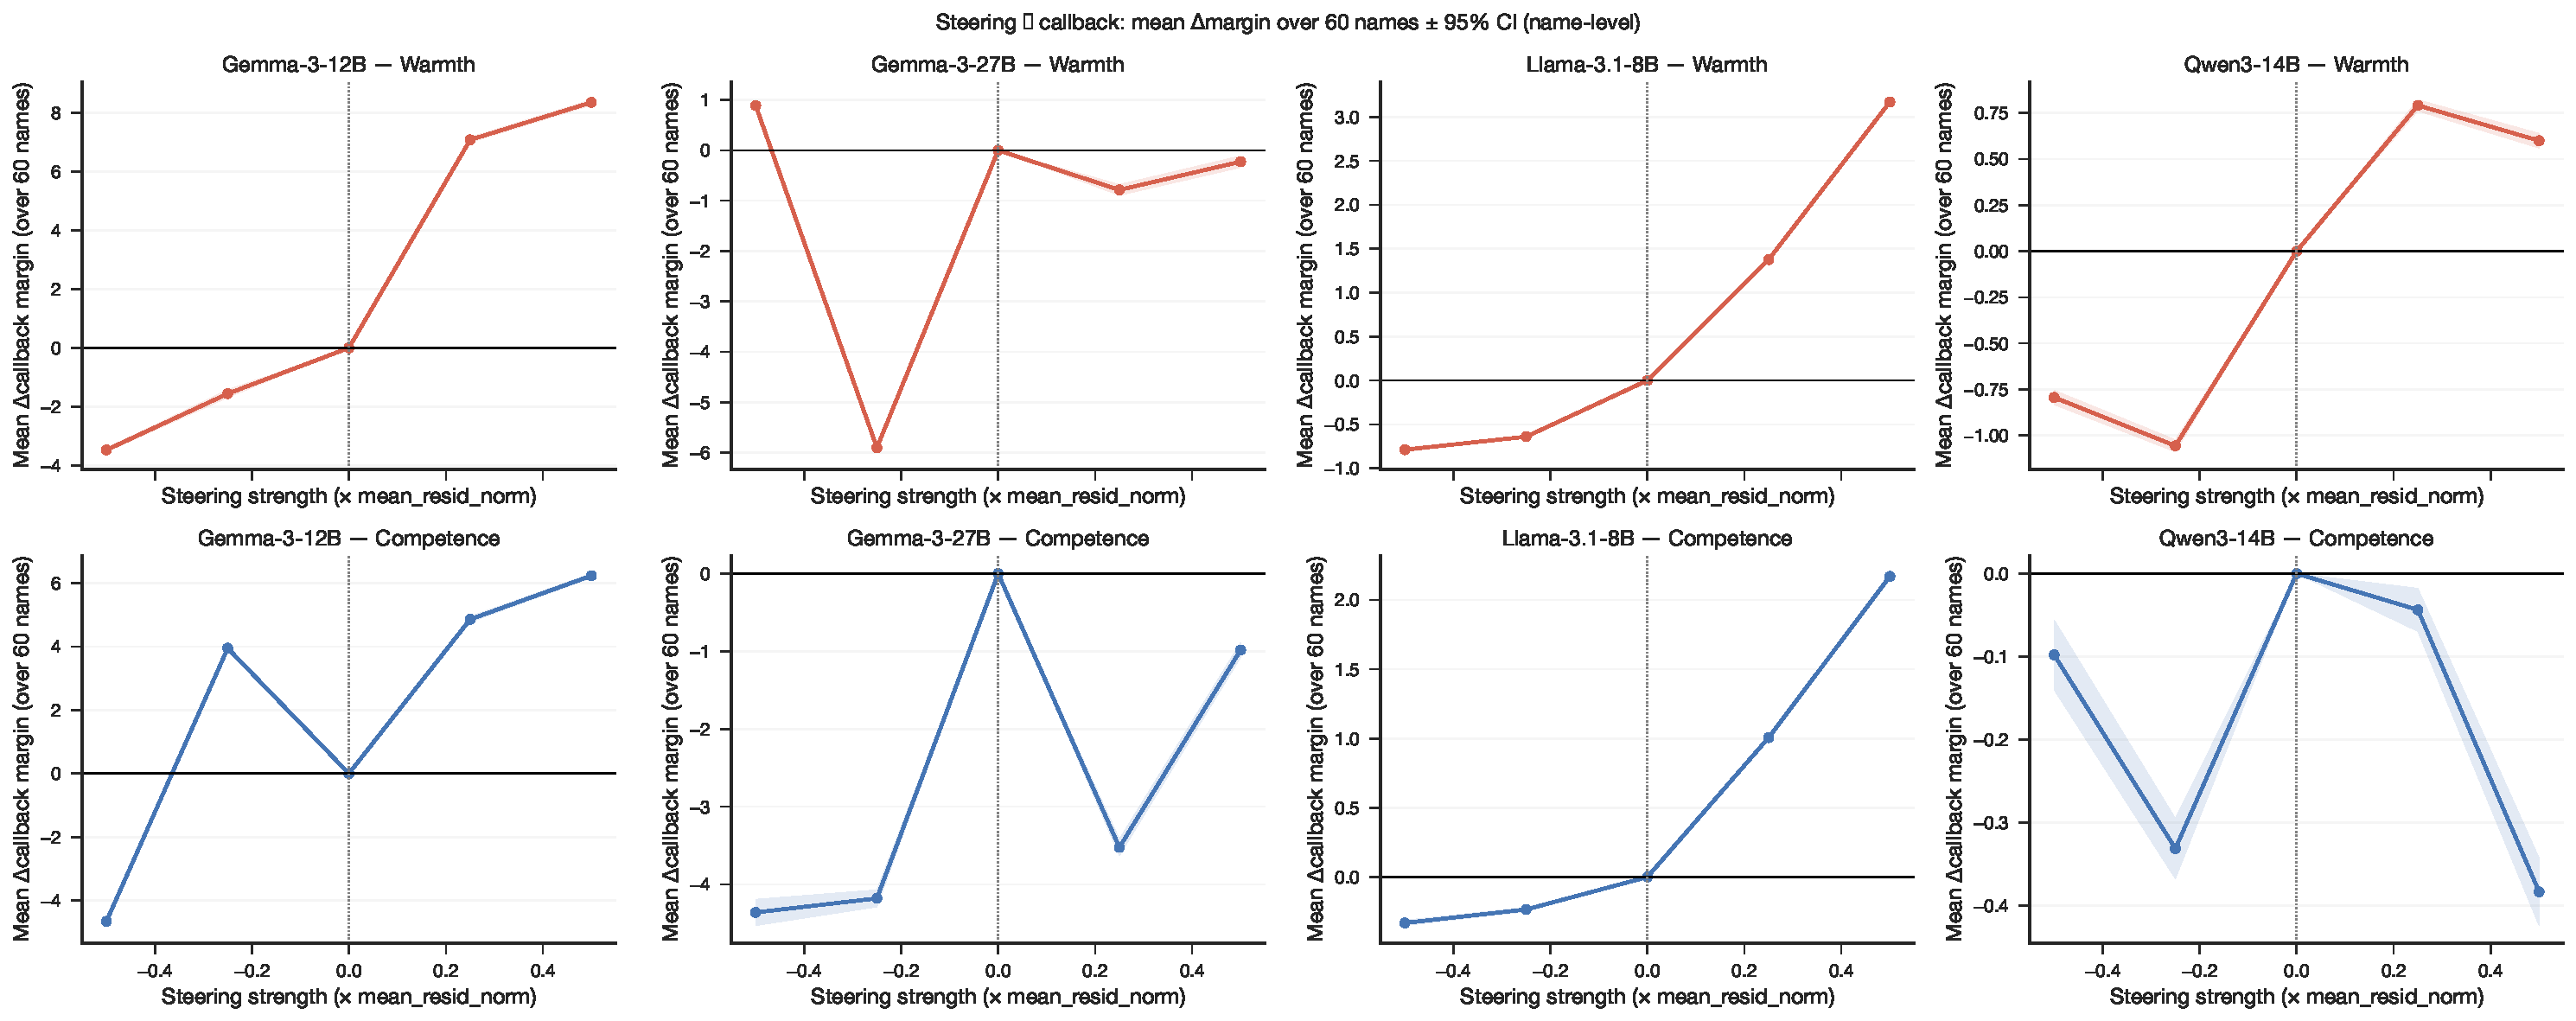
\includegraphics[width=\textwidth]{fig17_hiring_steering_callback.pdf}
\caption{\textbf{Activation steering işe alım callback önerilerini değiştirir.}
Hiring evaluation setting'inde warmth ve competence steering'e verilen
callback-margin response'ları.}
\label{fig:fig17_hiring_steering_callback}
\end{figure*}

\begin{figure*}[t]
\centering

\includegraphics[width=\textwidth]{fig13_dense_steering_doseresponse.pdf}
\caption{\textbf{Modeller arasında dense steering dose-response.}
Dört açık ağırlıklı modelde warmth ve competence direction'ları için
concept-level dose-response curve'leri.}
\label{fig:fig13_dense_steering_doseresponse}
\end{figure*}

\paragraph{Model Callback Disparity'leri ve Human Benchmark.}
Model hiring recommendation'larındaki demographic parity'yi human
correspondence-study outcome'larına göre değerlendirmek için 282-name stimulus
set'i, \citet{gallo2024warmth} çalışmasındaki yayımlanmış callback benchmark'a
first-name match üzerinden bağladık. 282 name'in 149'u eşleşti: 9 Black Female,
9 Black Male, 84 White Female ve 47 White Male. Human benchmark, klasik
audit-study pattern'ını gösterir: White name'ler Black name'lerden belirgin
ölçüde daha yüksek callback rate alır (race gap $= -0.085$, White lehine);
male name'ler de female name'lerden biraz daha yüksek rate alır (gender gap
$= -0.037$, Male lehine). Gemma-3-27B'de race gap human benchmark'a göre ters
ve büyüktür: Black-signalling name'lerin callback margin'ı White-signalling
name'lerden $+0.486$ raw logit unit daha yüksektir; bu değer $+1.18$ within-model
standard deviation'a eşittir (\autoref{fig:fig18_hiring_disparity}). 27B'deki
gender gap $-0.211$ raw logit unit'tir ($-0.51$ SD); human direction'ı
(Female $<$ Male) yeniden üretmekle birlikte human reference'tan daha büyüktür.
Bu sonuçlar büyük Gemma modelinin human racial discrimination pattern'ını
overcorrect ettiğini gösterir: Black-signalling name'lere empirical record'un
tersi yönde, büyük ve sistematik bir advantage verirken gender gap direction'ı
korur. Pattern, reinforcement learning from human feedback'in racial
association'ları öylesine güçlü düzeltmiş olmasıyla tutarlıdır ki ortaya çıkan
calibration, human outcome'ların empirical distribution'ını bir standard
deviation'dan fazla aşmıştır. Gemma-3-12B'de callback-margin variance group-level
disparity'leri güvenilir biçimde saptamak için çok düşüktür (SD $= 0.14$,
0.125 logit grid üzerinde yedi unique value); bu modelin R4 sonuçları
Limitations bölümünde açıklanmaktadır. Matched 149 name üzerinde modelin kendi
probe score'larından callback margin'ı yordayan exploratory ordinary
least-squares regression, warmth'ün 12B'de causal direction ile hizalandığını
(Pearson $r = +0.376$, $p < .001$), 27B'de ise tersine döndüğünü gösterir
($r = -0.266$, $p = .001$; $R^2 = 0.088$). Bu bulgu yukarıda belgelenen
reversed baseline association ile tutarlıdır. Llama-3.1-8B ve Qwen3-14B de
Black-signalling name'leri üstün tutar, ancak farklar daha küçüktür (within-model
SD cinsinden race gap sırasıyla $+0.40$ ve $+0.16$). İki model de female
name'lere male name'lerden daha yüksek margin verir ($+0.45$ ve $+0.89$ SD) ve
human gender direction'a karşı çıkar. Güvenilir margin variance'a sahip üç
modelin tamamı name'leri implied race ve gender'a göre farklı işler. Hiçbiri
human race direction'ı yeniden üretmez; human gender direction'ı yalnızca
Gemma-3-27B yeniden üretir. Dolayısıyla disparity pattern, kararlı biçimde
devralınmış bir bias değil, architecture ve scale'e bağlı bir yeniden
düzenlemedir.

\begin{figure*}[t]
\centering
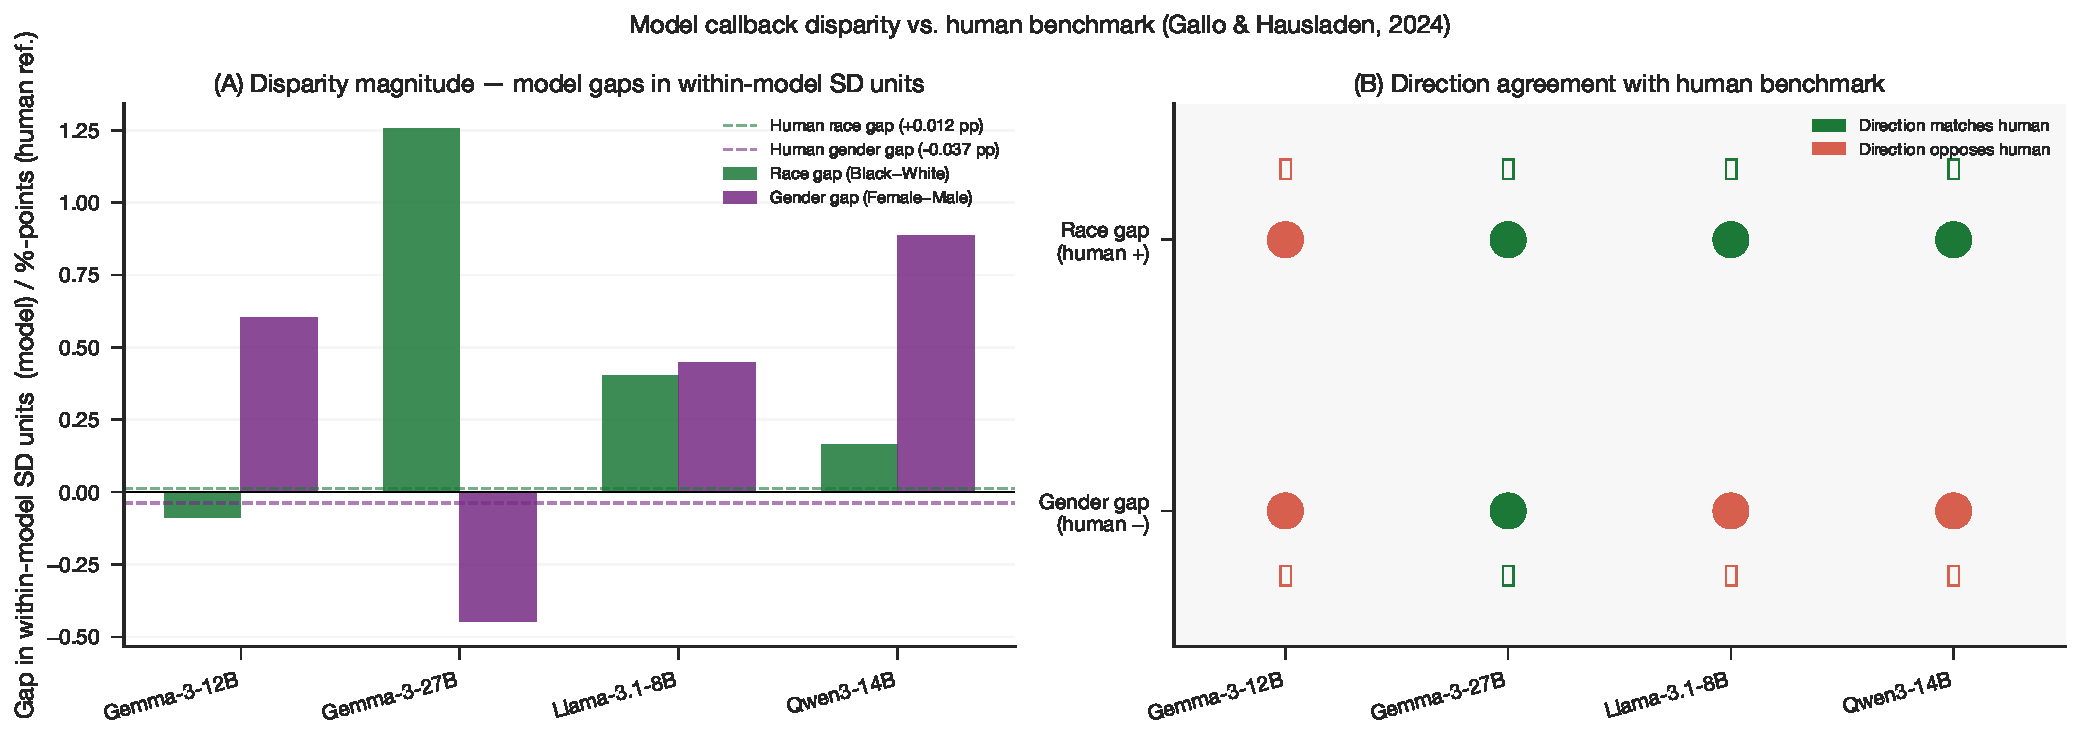
\includegraphics[width=\textwidth]{fig18_hiring_disparity.pdf}
\caption{\textbf{Human benchmark'a göre model callback disparity'leri.}
Model evaluation'lardaki race ve gender callback-margin gap'lerinin
correspondence-study benchmark ile karşılaştırılması.}
\label{fig:fig18_hiring_disparity}
\end{figure*}

\paragraph{Representation'lar, Steering'in En Zayıf Olduğu Yerde Disparity'ye Aracılık Eder.}
Name group $\to$ probe score $\to$ callback margin path'i üzerindeki bootstrap
mediation, steering'den farklı bir soruyu yanıtlar: external push'ın decision'ı
değiştirip değiştirmediğini değil, modelin bir name'e ilişkin spontaneous warmth
veya competence representation'ının demographic signal'ı callback outcome'a
taşıyıp taşımadığını sorar. On altı indirect effect'ten beşinin yüzde 95
interval'i zero'yu dışlar (\autoref{fig:fig19_hiring_mediation_forest}).
Llama-3.1-8B'de race disparity warmth üzerinden mediate edilir
(IE $= +0.190$, yüzde 95 CI $[+0.111, +0.292]$) ve competence üzerinden daha
zayıf bir mediation görülür ($+0.040$, $[+0.004, +0.090]$). Qwen3-14B'de race,
warmth üzerinden positive ($+0.081$), competence üzerinden negative
($-0.132$) mediate edilir; gender ise competence üzerinden positive mediate
edilir ($+0.076$). İki Gemma modeli için sekiz testin tamamı non-significant'tır.
On altı test multiple-comparison correction olmadan raporlanmıştır; yalnızca
Llama race--warmth path konservatif Bonferroni threshold'unu
($\alpha = 0.05/16$) geçer. Bu nedenle daha küçük significant effect'ler
suggestive olarak okunmalıdır. Steerability ranking ile birlikte bu sonuçlar bir
\textit{steerability paradox} oluşturur: Suite'teki en steerable model olan
Gemma-3-12B (normalized warmth steerability $0.236$) significant mediation path
göstermezken, en az steerable model Llama-3.1-8B ($0.029$) en güçlü path'i
gösterir. Bir representation'ı external push ile değiştirme kapasitesi, o
representation'ın downstream decision'ı doğal olarak yönetip yönetmediğini
yordamamaktadır. Steering intervention'a causal sensitivity'yi, mediation ise
natural activation'ın outcome'a taşınıp taşınmadığını ölçer; bu iki ölçüm
architecture'lar arasında dissociate olur.

\begin{figure*}[t]
\centering
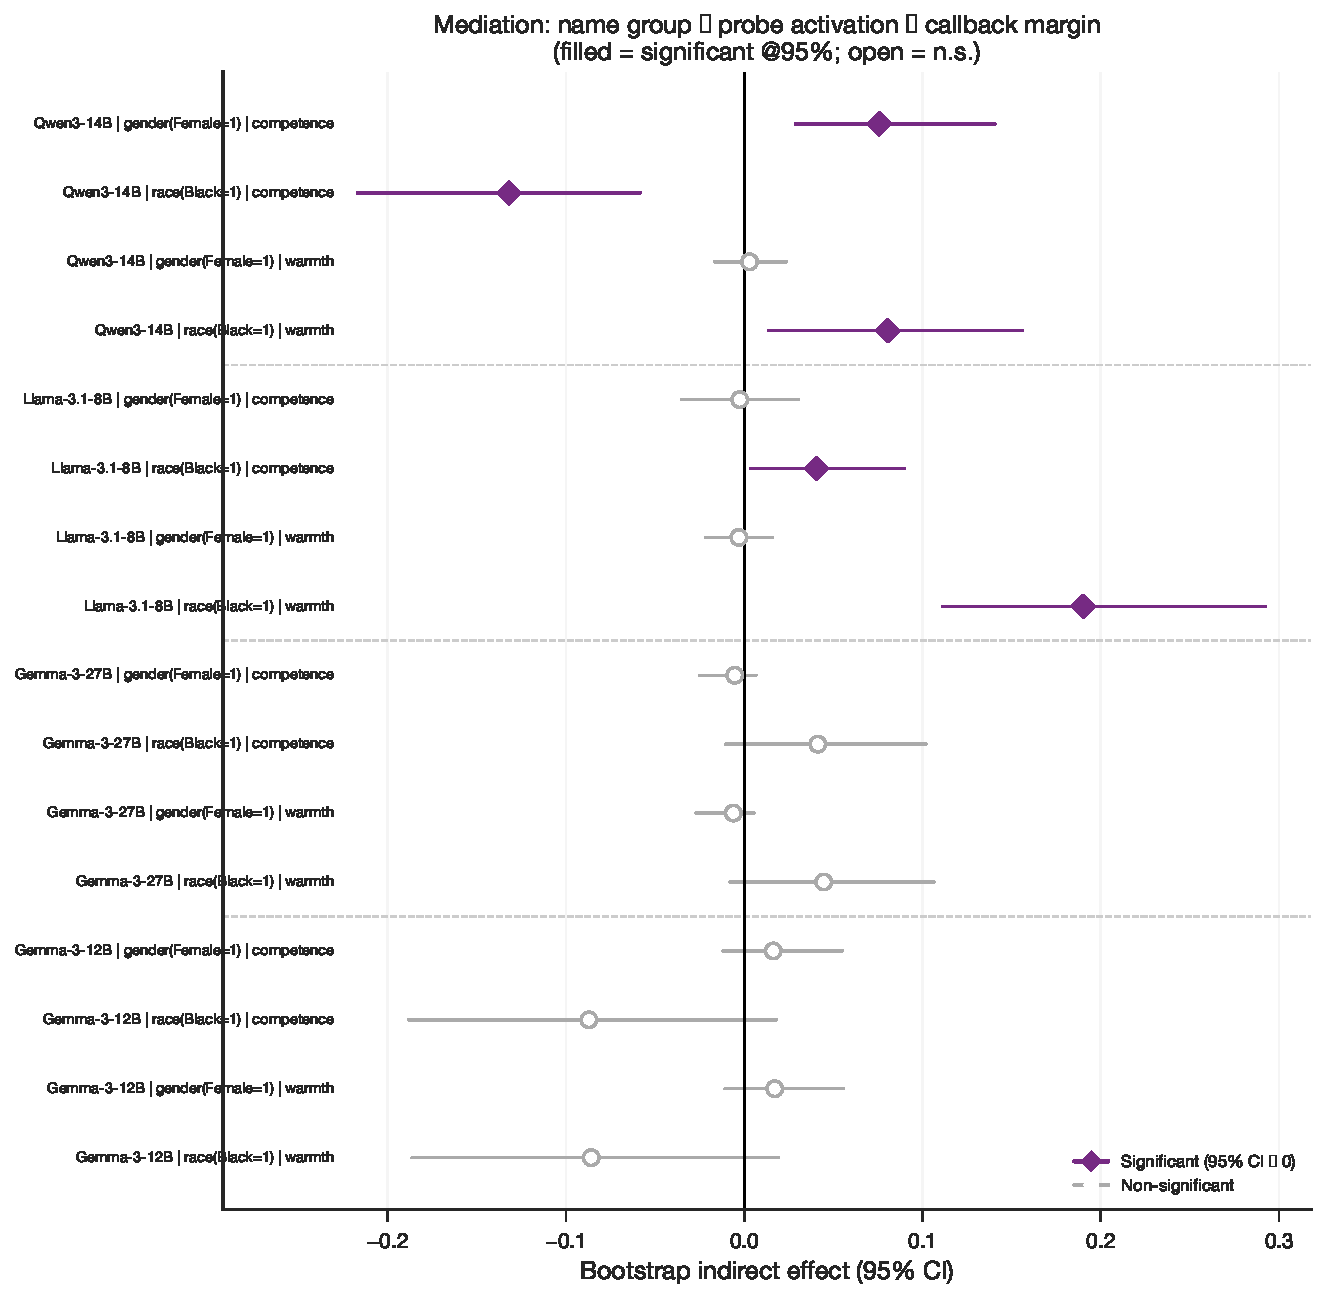
\includegraphics[width=\textwidth]{fig19_hiring_mediation_forest.pdf}
\caption{\textbf{Name-group callback disparity'lerinin warmth ve competence probe score'ları üzerinden bootstrap mediation'ı.}
Name group $\to$ probe score $\to$ callback margin path'i için yüzde 95
confidence interval içeren indirect effect'ler; dolu marker'lar zero'yu dışlayan
interval'leri gösterir.}
\label{fig:fig19_hiring_mediation_forest}
\end{figure*}

% -----------------------------------------------------------------------------
\section*{Tartışma ve Sonuç}
% -----------------------------------------------------------------------------

İnsanlar tarafından üretilmiş text üzerinde train edilen large language
model'lerin warmth ve competence'ı içeriden çıkarılabilir representation'lar
olarak kodlaması bir açıdan şaşırtıcı değildir; bu modeller, warmth ve
competence'ın social perception'ı şekillendirdiği aynı text'lerdeki pattern'ları
damıtır. Mevcut sonuçların ampirik olarak ortaya koyduğu nokta, bu encoding'in
linear, geometrically stable, concept level'da causally functional ve bağımsız
laboratory'lerde geliştirilmiş mimari açıdan farklı modeller arasında shared
olmasıdır. Bu özelliklerin her biri önem taşır: linearity, representation'ı
lightweight probe ve steering intervention'larına erişilebilir kılar; causal
functionality, representation'ın warmth ve competence'a ilişkin explicit
judgement'lara katıldığını gösterir; cross-architecture convergence ise
finding'in tek bir design'a özgü olmaktan çok training data ve language
modelling objective'lerinin bir özelliğini yansıttığını düşündürür.

Gemma-3-12B ile Gemma-3-27B arasındaki scale comparison, bu görünümü öğretici
biçimde karmaşıklaştırır. İki model de warmth ve competence'ı karşılaştırılabilir
precision ile kodlar; 27B modelinin probe score'ları human warmth ve competence
rating'leriyle biraz daha güçlü correlate olur. Buna karşılık concept
representation'dan hiring decision'a uzanan causal chain iki model arasında
keskin biçimde ayrışır. 12B'de warmth representation'ı artırmak callback
inclination'da büyük ve yaklaşık linear bir artış üretir ($\alpha = +0.10$
düzeyinde $+2.37$ logit unit'e kadar). 27B'de eşdeğer intervention düşük
strength'te modest positive shift üretir ($\alpha = +0.05$ düzeyinde $+1.97$),
ancak biraz daha yüksek strength'te büyük negative shift'e çöker
($\alpha = +0.10$ düzeyinde $-2.66$). Bu non-monotone response saturation
değildir: 27B baseline zaten $P(\text{Yes}) = 0.76$ düzeyindedir ve upward
movement için alan bırakır; response plateau değil sign reversal'dır. Daha
plausible açıklama, 27B decision layer'ın birbiriyle etkileşen birden çok
representation tarafından organize edilmesidir. Concept direction dar bir
window'un ötesinde amplify edildiğinde bu etkileşimleri güçlendirmek yerine
bozmaya başlar.

Cross-model steerability analysis ile bağlantılı başka bir puzzle ortaya çıkar.
Gemma-3-12B en yüksek concept steerability değerine sahiptir (normalized warmth
steerability $= 0.236$), fakat significant bir hiring-level mediation path
göstermez. Llama-3.1-8B en düşük concept steerability değerine sahiptir
(normalized warmth steerability $= 0.029$) ve en güçlü hiring-level indirect
effect'i gösterir (bootstrap IE $= +0.190$). Bu steerability paradox, bir modelin
representation'larını linear probing yoluyla değiştirme kapasitesinin, bu
representation'ların downstream decision'ı nedensel olarak yönettiği anlamına
gelmediğini gösterir. Representation'ların en temiz biçimde izole edilebildiği
modeller, decision process'in steering target'ı bypass eden parallel mechanism'lar
üzerinden çalıştığı modeller olabilir.

Llama-3.1-8B ve Qwen3-14B'de gözlenen warmth anti-alignment ek bir complexity
katmanı oluşturur. Yüksek cross-model story agreement'a rağmen (Gemma ile diğer
iki model arasında per-story Spearman $\rho \approx 0.76$--$0.77$), Llama ve
Qwen'in activation space içinde ``high warmth'' olarak düzenlediği direction,
human warmth rating'leriyle negative correlate olur (sırasıyla $\rho = -0.300$
ve $-0.193$). Modeller story'lerin aynı relative ordering'i üzerinde birleşir,
fakat bu ortak ordering human scale'e göre terstir. Bunu, instruction tuning'in
bu architecture'lardaki warmth axis'i yeniden yapılandırdığına dair kanıt olarak
yorumluyoruz. Reinforcement learning from human feedback, stereotypically warm
social group'larla ilişkilendirilen representation'ları, original pretraining
warmth axis'iyle bağlantıyı tersine çevirecek biçimde ayarlamış olabilir.

Gemma-3-27B'deki demographic disparity sonuçları bu representational
reorganization'ın pratik sonucunu gösterir. Model, Black-signalling name'lere
White-signalling name'lere göre güçlü bir advantage sağlar ($+1.18$ SD) ve
klasik correspondence-study finding'ini doğrudan tersine çevirir. Buna karşılık
gender gap direction human pattern'ı yeniden üretir. Race ve gender arasındaki
asymmetry, instruction tuning'in farklı demographic axis'lere farklı
correction'lar uyguladığını düşündürür. Ortaya çıkan model overall daha
equitable değil, farklı biçimde inequitable'dır: racial hierarchy ortadan
kalkmak yerine tersine dönmüş ve original human disparity'den çok daha büyük
bir magnitude'a ulaşmıştır. Bu finding, outcome-level bias mitigation'ın temel
bir sınırlılığına işaret eder. Representational substrate anlaşılmadan
behavioral output'ları düzeltmek, underlying imbalance'ı kaldırmak yerine başka
bir yöne kaydırabilir.

Sonuçlar birlikte değerlendirildiğinde LLM'lerin, explicit bir design choice
olmaksızın human-generated text üzerinde training yoluyla SCM'ye geniş ölçüde
benzeyen bir social perception structure'ı içselleştirdiği görülür. Bununla
birlikte bu iç structure ile actual hiring decision arasındaki bağlantı basit
ya da modeller arasında tutarlı değildir. Bu finding, bias auditing için
methodological bir sonuç doğurur: internal representation'ları probing ile
incelemek ve output disparity'lerini ölçmek birbirini tamamlar, ancak birbirinin
yerini tutmaz; bir metric'te iyi performans gösteren model diğerinde aynı sonucu
vermeyebilir. Çalışma ayrıca, output'ları sonradan filter etmek yerine
representation'a müdahale ederek problemi kaynağında ele alma yolu açmakta ve
mechanistic interpretability'nin computational tool'larını social science'taki
correspondence-study geleneğiyle birleştiren bir methodological template
sunmaktadır.

\paragraph{Sınırlılıklar.}
Concept story corpus'un bir large language model tarafından üretilmiş olması,
language model representation'larını probing ile inceleyen bir çalışma için
circularity endişesi doğurur. Bununla birlikte generating model (Claude,
Anthropic) ile probing uygulanan modeller (Gemma, Qwen, Llama) farklı
organization ve architecture'lardan gelir; dolayısıyla warmth/competence
contrast'ları shared generator tarafından trivially yeniden üretilmez. Yine de
AI-generated stimulus'ların model aileleri arasında probe accuracy'yi yükselten
ortak stylistic property'lere sahip olma olasılığı tümüyle dışlanamaz;
human-authored veya template-based stimulus'larla replication yapılması yararlı
olacaktır. Mevcut 200 story'lik corpus, 50 topic'i kapsayan bir pilot'tur;
planlanan 400 story'lik expansion, per-condition sample size ve topic diversity'yi
artıracaktır. Probe-to-human validation correlation'ları moderate düzeydedir
(12B ve 27B için warmth $\rho = +0.366$ ve $+0.396$; competence
$\rho = +0.239$ ve $+0.272$). Bu değerler, modelin internal probe'larının human
social perception'ı birebir yeniden üretmek yerine onun bir component'ini
yakaladığını gösterir. Llama-3.1-8B ($\rho = -0.300$) ve Qwen3-14B'deki
($\rho = -0.193$) warmth anti-alignment, bu modellerde mean-difference
direction'ın human warmth scale'e göre sistematik biçimde ters bir construct'ı
yakaladığı anlamına gelir; sonuçlar bu inversion dikkate alınarak
yorumlanmalıdır. Hiring level'daki causal warmth steering effect 12B'de positive
ve güçlü, 27B'de ise non-monotone ve kırılgandır. Bu nedenle causal claim,
qualification olmadan scale boyunca genellenemez. Model output logit'lerindeki
bf16 precision nedeniyle callback margin'lar 0.125-unit grid üzerinde quantized
edilmiştir; bu quantization bf16 inference'a özgüdür ve float32 subtraction ile
çözülmez. Gemma-3-12B'de callback-margin standard deviation 0,14 ve unique value
sayısı yalnızca yedidir. Bu nedenle 12B'deki group-level disparity estimate'leri
güvenilir değildir ve 12B R4 sonuçları empirical finding olarak cite
edilmemelidir. Gemma-3-27B'de daha büyük variance (SD $= 0.41$, 18 unique value),
yaklaşık 0,5 SD büyüklüğündeki group gap'lerin saptanmasını mümkün kılar; ancak
grid structure raporlanan bütün gap magnitude'larına discrete step'ler ekler.
On altı mediation test, multiple comparison correction olmadan sunulmuştur;
yalnızca Llama race--warmth indirect effect Bonferroni-corrected threshold'u
geçer. Daha küçük significant path'ler doğrulanmış değil suggestive kabul
edilmelidir. Hiring prompt gerçek dünyadaki screening context'lerine göre
basitleştirilmiştir (tek role, sabit qualification); daha zengin evaluation
setting'lerinde veya farklı job type'larda sonuçlar değişebilir. Son olarak,
Gemma-3'te Qwen3 ve Llama-3.1'e kıyasla bütün network depth'lerinde gözlenen
yüksek warmth/competence vector cosine'ın architectural kaynağı açık bir soru
olarak kalmaktadır.

\paragraph{Gelecek Çalışmalar.}
İlk adım, sonuçların administrative assistant role'ünün ötesine genellenip
genellenmediğini test etmek için hiring stimulus'larını farklı job role'lerine
genişletmektir. Burada Gemma-3 üzerinde gerçekleştirilen SAE decomposition,
Llama Scope sparse autoencoder'ları \citep{lindsey2025llama} kullanılarak
Llama-3.1'e genişletilebilir ve feature level'da model-family comparison
yapılabilir. Concept probe'larının human-authored warmth/competence dataset ile
validation'ı, AI-generated stimulus'larla ilişkili circularity endişesini ele
alacaktır. Social-science tarafında hiring stimulus'larını name'lerin ötesinde
category-level signal'lara (age, disability, religion) genişletmek, benchmark
comparison'ın scope'unu büyütür ve representational account'ın race ile gender
dışında genellenip genellenmediğini test eder. Bu finding'leri practical
debiasing intervention'larına dönüştürmek ve adversarial prompting'e karşı
robustness'larını değerlendirmek applied work için doğal bir sonraki adımdır.

{
\footnotesize
\setlength{\bibitemsep}{-0.5ex}

\clearpage
\section*{Kaynakça}
\begin{otherlanguage}{english}
\printbibliography[heading=none]
\end{otherlanguage}
}

\clearpage
\begin{appendices}
\onecolumn
\setcounter{figure}{0}
\setcounter{table}{0}
\renewcommand{\thesection}{\Alph{section}}%
\renewcommand{\thesubsection}{\thesection.\arabic{subsection}}
\renewcommand\thefigure{S.\arabic{figure}}
\renewcommand\thetable{S.\arabic{table}}
\begin{center}
    \begin{minipage}{\textwidth}
        \centering
        \fontsize{16}{20}\selectfont
        Ek Materyaller
    \end{minipage}
\end{center}
\vspace{.5cm}

\section*{Yöntem Ayrıntıları}
\label{apx:methods}

\section*{Ek Bulgular}

\end{appendices}
\end{document}
